\subsection{Visitor Pattern und Double Dispatch}


\subsubsection*{Problembeschreibung}

Gelegentlich muss eine Operation auf einer Menge von Objekten durchgeführt, die alle Teil einer Objekthierarchie aber unterschiedlich sind. Diese Objekte besitzen daher unter Umständen voneinander abweichende Schnittstellen. Das \emph{Visitor Pattern} erlaubt es, solche Operationen außerhalb der Objekte und für alle betroffenen Objekte innerhalb einer separaten Klasse zu definieren. \cite{gamma_design_1995}

\subsubsection*{Lösung}

Der konkrete \emph{Visitor}\footnote{Die deutsche Übersetzung ''Besucher'' ist in diesem Kontext eher unüblich.} (\code{ConcreteVisitor}) realisiert die \emph{Visitor}-Schnittstelle (\code{Visitor}), welche die Methode \code{visit} bereitstellt, wie in \autoref{fig:visitor-class} zu erkennen ist. Diese erlaubt es dem \emph{Visitor}, ein Element (\code{Element}) zu ''besuchen'' und auf ihm eine Operation durchzuführen. Die Elemente ''akzeptieren'' den ''Besuch'' des \emph{Visitors} mithilfe der Methode \code{accept}, welche als Argument den besuchenden \emph{Visitor} erhält.

\begin{figure}[!ht]
	\centering
	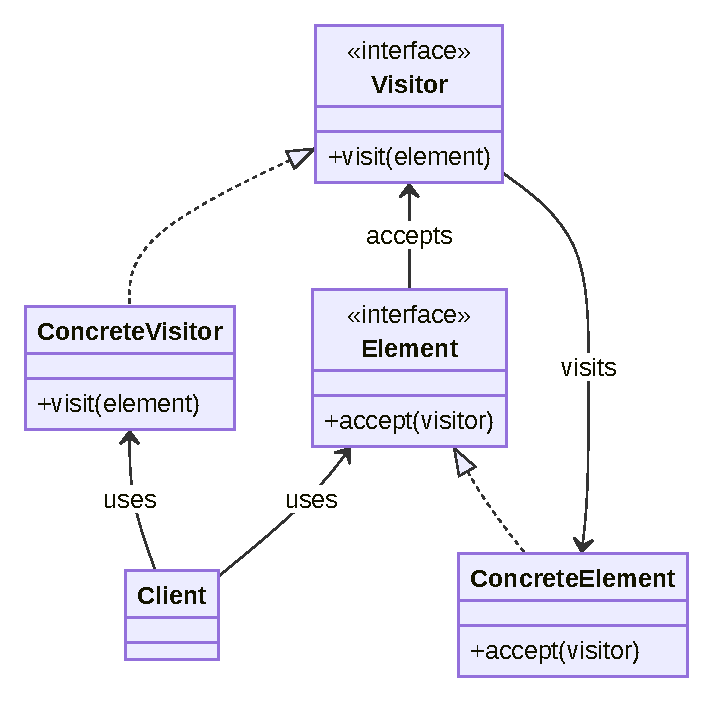
\includegraphics[width=0.75\linewidth]{images/patterns/visitor-class.pdf}
	\caption{Klassendiagramm des \emph{Visitor Patterns}. Der \code{Visitor} kapselt eine Operation auf einer Menge von Elementen in seinen \code{visit}-Methoden. Die Elemente werden von dem \code{Visitor} ''besucht'' und rufen die zu ihrem Typ korrespondierende Methode auf dem Visitor auf. \cite{skobeleva_visitor_2023}}
	\label{fig:visitor-class}
\end{figure}

\autoref{fig:visitor-seq} zeigt das Verhalten des \emph{Visitor Patterns}. Der Anwender\footref{ftn:client} trägt dem \emph{Visitor} auf, eine Operation auf einem Element oder einer Menge von Elementen durchzuführen (1). Der \emph{Visitor} sendet daraufhin \code{visit} an alle Elemente, auf die er eine Referenz hält (2). Jedes Element ruft daraufhin eine \code{accept}-Methode auf dem \emph{Visitor} auf (3). Zu beachten ist hierbei, dass es für jede Element-Klasse eine eigene Methode im \emph{Visitor} gibt. Dies kann realisiert werden durch das Bereitstellen von Methoden mit unterschiedlichen, zu den aufrufenden Klassen korrespondierenden Namen oder durch Multimethoden. Multimethoden sind Methoden, welche je nach Typ der übergebenen Argumente unterschiedliche Implementierungen ausführen. Somit kann der \emph{Visitor} nach Erhalt von \code{accept} die zum Typ des sendenden Elements passende Operation ausführen. Dieser Mechanismus nennt sich \emph{Double Dispatch}.

\begin{figure}[!ht]
	\centering
	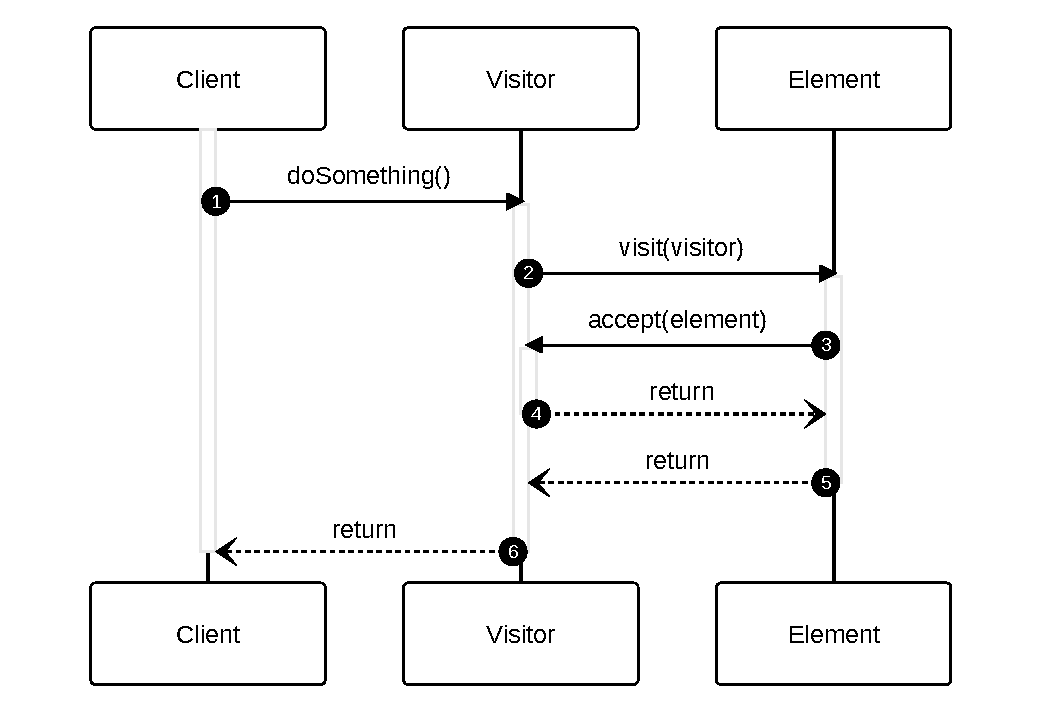
\includegraphics[width=0.75\linewidth]{images/patterns/visitor-seq.pdf}
	\caption{Sequenzdiagramm des \emph{Visitor Patterns}. Das Entwurfsmuster nutzt einen \emph{Double Dispatch}, um die Ausführung der korrekten Methode im \code{Visitor}-Objekt zu gewährleisten. Dazu ruft der Visitor auf dem Element die Methode \code{accept} auf (2). Diese ruft dann die zum Element passende \code{visit}-Methode auf (3). \cite{skobeleva_visitor_2023}}
	\label{fig:visitor-seq}
\end{figure}

\subsubsection*{Konsequenzen}
Durch die Kapselung der Operation in einem \emph{Visitor}, ist es sehr einfach, neue Operationen hinzuzufügen. Es bedarf dazu lediglich eines weiteren \emph{Visitors}. Außerdem kapselt ein \emph{Visitor} die Menge an Operationen auf den Elementen. Zusammengehörige Operationen werden in einer Klasse gesammelt. Nicht zueinander gehörende Operationen befinden sich in unterschiedlichen \emph{Visitors}. Ein weiterer Vorteil eines \emph{Visitors} ist dessen Fähigkeit, während des ''Besuchens'' mehrerer Elemente Informationen über diese zu akkumulieren und im Anschluss gebündelt zu repräsentieren.

Der \emph{Visitor} weist jedoch auch Nachteile auf. Zum einen ist es schwer, weitere konkrete Element-Klassen zu einem System hinzuzufügen, welches bereits eine Reihe an \emph{Visitors} besitzt. Da ein \emph{Visitor} für jeden Typ von Element eine Methode bereitstellen muss, kann ein weiteres Element einen erhöhten Implementierungsaufwand bedeuten. Das \emph{Visitor Pattern} sollte daher nur verwendet werden, wenn entweder die Menge an Elementklassen abgeschlossen oder die Menge an \emph{Visitor}-Klassen übersichtlich ist. Zum anderen müssen die Elemente dem \emph{Visitor} eine Schnittstelle bereitstellen, welche es dem \emph{Visitor} ermöglicht, seine Operation ausführen zu können. Dies kann dazu führen, dass das Element einen großen Teil seines internen Zustands preisgeben muss, welcher bei nicht-Verwendung dieses Musters gekapselt geblieben wäre. \cite{gamma_design_1995}